% **********************
% Appendix A: multipoles
% **********************

\chapter{Multipole analysis of the MW effect on Andromeda}

In this section, the contribution of each of the components of the multipolar expansion of the MW (under different models) is analyzed in order to determine if the distribution of dark matter can produce detectable effects at the distance of the Andromeda galaxy (M31).

% **********************
% Section on the multipole expansion
% **********************

\section{Multipole expansion of the gravitational potential}

The general expression for the gravitational potential produced by a distribution $U$ on a point $\vec{r}$ (see figure \ref{fig:potential_scheme}) is given by:

\begin{figure}
    \label{fig:potential_scheme}
    \centering
    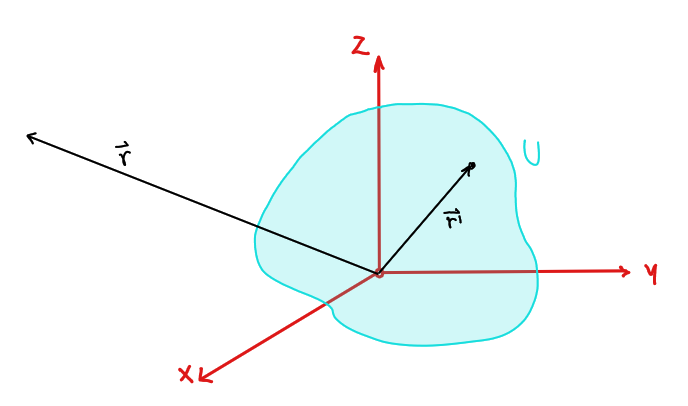
\includegraphics[scale=0.4]{potential_scheme.png}
    \caption{Scheme of the mass distribution $U$ generating a potential on $\vec{r}$}
    \label{fig:my_label}
\end{figure}

\begin{equation}\label{eq:pot_def}
    \phi (\vec{r}) = -G\int\displaylimits_U \
    \frac{\rho(\vec{r^\prime})}{|\vec{r}-\vec{r^\prime}|} \ 
    \mathrm{d}V^\prime
\end{equation}

The integrand can be expanded using the Legendre polynomials, and considering the addition theorem, the expansion can be brought to the following form \cite{arfken_ed7_chap16}:

\begin{equation*}
    \frac{1}{|\vec{r}-\vec{r^\prime}|} = \ 
    \sum\displaylimits_{l=0}^{\infty} \frac{{r_<}^l}{{r_>}^{l+1}} \ 
    \sum\displaylimits_{m=-l}^{l} {Y_l}^m(\Omega)^*{Y_l}^m(\Omega^\prime)
\end{equation*}

Where $r_<$ and $r_>$ are, respectively, the smaller and larger of $r$ and $r^\prime$, ${Y_l}^m$ are the spherical harmonics, and $\Sigma$ and $\Sigma^\prime$ are the angular coordinates of $r$ and $r^\prime$.

In the situations of interest, the potential only needs to be known considerably far away from the mass distribution that produces it. Because of this, is clear that $r>r^\prime$, so the expansion is just:

\begin{equation}\label{eq:exp_legendre}
    \frac{1}{|\vec{r}-\vec{r^\prime}|} = \ 
    \sum\displaylimits_{l=0}^{\infty} \frac{{r^\prime}^l}{{r}^{l+1}} \ 
    \sum\displaylimits_{m=-l}^{l} {Y_l}^m(\Omega)^*{Y_l}^m(\Omega^\prime)
\end{equation}

Considering \ref{eq:exp_legendre} in \ref{eq:pot_def}, the multipole expansion of the gravitational potential therefore is:

\begin{equation}\label{eq:pot_multipole}
    \boxed{\phi = - G \sum\displaylimits_{l=0}^{\infty} \ 
    \sum\displaylimits_{m=-l}^{l} {M_l}^m \ 
    \frac{{Y_l}^m(\Omega)^*}{r^{l+1}}}
\end{equation}

And the multipole moments, ${M_{l}}^{m}$, are defined as:

\begin{equation}\label{eq:multipole_moments}
    \boxed{{M_l}^{m} = \frac{4\pi}{2l+1}\int\displaylimits_{U} \ 
    {r^\prime}^l \rho(\vec{{r^\prime}}) {Y_l}^m(\Omega^\prime) \ 
    \mathrm{d}V^\prime}
\end{equation}

\subsection{Linearity of the multipole moments}

When analyzing the mass density distribution of the source, is common to describe the density as a superposition of the density of different components of the system (e.g. $\rho_{disk}(\vec{r})$, $\rho_{bulge}(\vec{r})$, $\rho_{halo}(\vec{r})$). In this case, because of the linearity of the integrals, the multipole moments are also linear in $\rho$

\section{Multipole expansion of the gravitational field}



% ************************
% Sections on the different models for the MW
% ************************

\section{Models for the MW}

To measure the contribution of the components and the effect of different types of halos, a set of models will be compared. This models will be:

\begin{enumerate}
    \item disk + bulge
    \item disk + bulge + spherical halo
    \item disk + bulge + ellipsoidal halo
\end{enumerate}

\subsection{disk + bulge}

\subsection{disk + bulge + spherical halo}

\subsection{disk + bulge + ellipsoidal halo}

